\usetikzlibrary{snakes}

\begin{figure}[tb]
    \centering
    
    
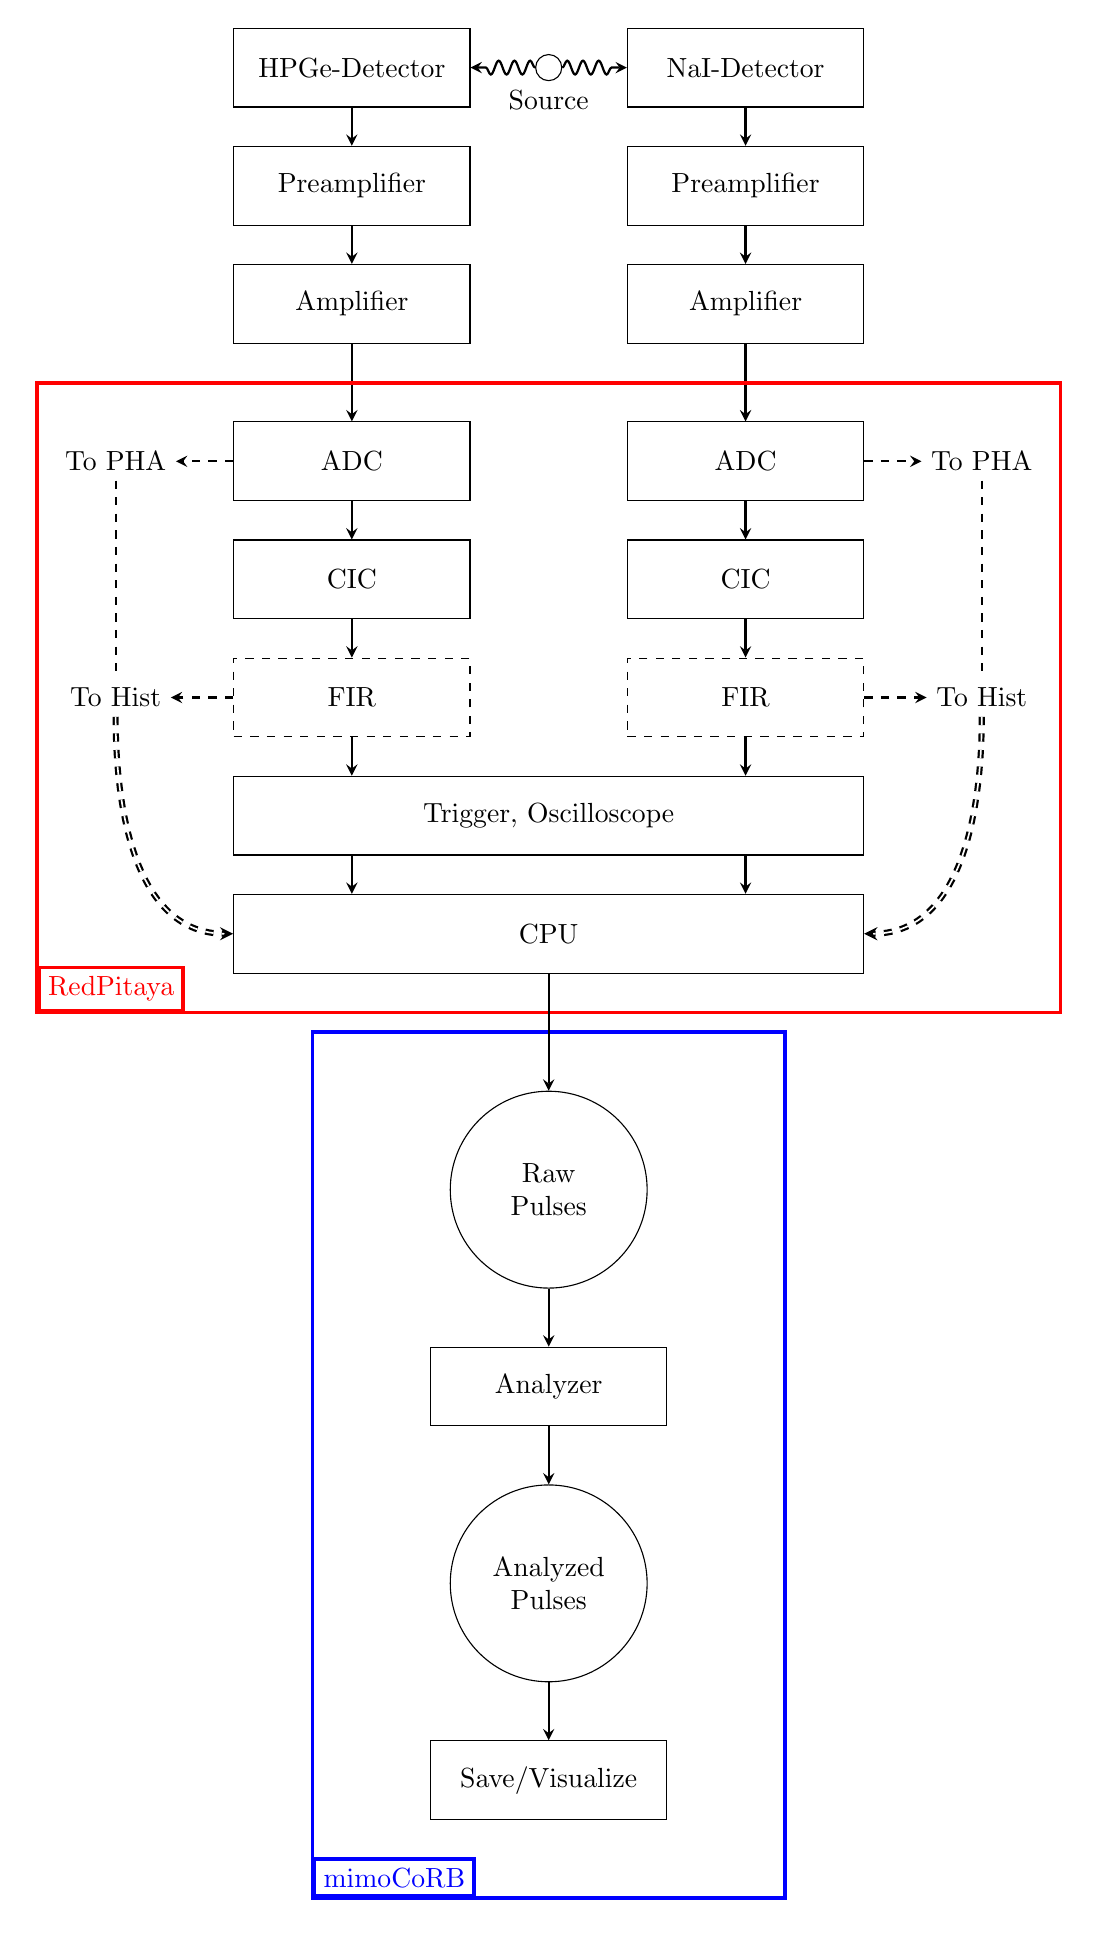
\begin{tikzpicture}[node distance=1.5cm]
\tikzstyle{Module} = [rectangle,  minimum width=3cm, minimum height=1cm,align=center, draw=black]
\tikzstyle{ModuleDummy} = [rectangle,  minimum width=3cm, minimum height=1cm,text centered, draw=none]
\tikzstyle{Trash} = [rectangle, minimum width=1cm, draw=none]
\tikzstyle{source} = [circle, text centered, minimum size=.2cm, draw=black, label=below:{Source}]
\tikzstyle{Both} = [rectangle, minimum width=8cm, minimum height=1cm,text centered, draw=black]

\tikzstyle{RB} = [circle, align=center, minimum size=2.5cm, draw=black]

\tikzstyle{arrow} = [thick,->,>=stealth]
\tikzstyle{line} = [thick]


\def\xsep{4cm}


\def\xtrash{1.5cm}


\node (source) [source] at (0,0) {};

\node[Module, right of =source, xshift=1cm] (Na) {NaI-Detector};
\node[Module, left of =source, xshift=-1cm] (Ge) {HPGe-Detector};


\draw[arrow,decorate, decoration={snake, segment length=2mm, post length=1.5mm}] (source) -- (Na);
\draw[arrow,decorate, decoration={snake, segment length=2mm, post length=1.5mm, mirror}] (source) -- (Ge);

\node[Module, below of =Na] (NPreAmp) {Preamplifier};
\node[Module, below of =Ge] (GPreAmp) {Preamplifier};
\draw[arrow] (Na) -- (NPreAmp);
\draw[arrow] (Ge) -- (GPreAmp);

\node[Module, below of =NPreAmp] (NAmp) {Amplifier};
\node[Module, below of =GPreAmp] (GAmp) {Amplifier};
\draw[arrow] (NPreAmp) -- (NAmp);
\draw[arrow] (GPreAmp) -- (GAmp);




\node[Module, below of =NAmp, yshift=-.5cm] (NADC) {ADC};
\node[Module, below of =GAmp, yshift=-.5cm] (GADC) {ADC};
\draw[arrow] (NAmp) -- (NADC);
\draw[arrow] (GAmp) -- (GADC);



\node[Module, below of =NADC] (NCIC) {CIC};
\node[Module, below of =GADC] (GCIC) {CIC};
\draw[arrow] (NADC) -- (NCIC);
\draw[arrow] (GADC) -- (GCIC);

\node[Module, below of =NCIC, dashed] (NFIR) {FIR};
\node[Module, below of =GCIC, dashed] (GFIR) {FIR};
\draw[arrow] (NCIC) -- (NFIR);
\draw[arrow] (GCIC) -- (GFIR);



\node[ModuleDummy, below of=NFIR] (NTrigOsc) {};
\node[ModuleDummy, below of=GFIR] (GTrigOsc) {};
\draw[arrow] (NFIR) -- (NTrigOsc);
\draw[arrow] (GFIR) -- (GTrigOsc);

\node[Both, below of =source, yshift=-8cm] (TrigOsc) {Trigger, Oscilloscope};
\node[Both, below of =TrigOsc] (CPU) {CPU};

\node[ModuleDummy, below of=NTrigOsc] (NCPU) {};
\node[ModuleDummy, below of=GTrigOsc] (GCPU) {};
\draw[arrow] (NTrigOsc) -- (NCPU);
\draw[arrow] (GTrigOsc) -- (GCPU);

% Trash
\node[Trash, right of=NADC, xshift=+\xtrash] (NPHA) {To PHA};
\node[Trash, left of=GADC, xshift=-\xtrash] (GPHA) {To PHA};
\draw[arrow, dashed] (NADC) -- (NPHA);
\draw[arrow, dashed] (GADC) -- (GPHA);

\node[Trash, right of=NFIR, xshift=+\xtrash] (NHist) {To Hist};
\node[Trash, left of=GFIR, xshift=-\xtrash] (GHist) {To Hist};
\draw[arrow, dashed] (NFIR) -- (NHist);
\draw[arrow, dashed] (GFIR) -- (GHist);

\node[Trash, right of=NCPU, xshift=+\xtrash] (NTrash) {};
\node[Trash, left of=GCPU, xshift=-\xtrash] (GTrash) {};
\draw[line, dashed] (NPHA) -- (NHist);
\draw[line, dashed] (GPHA) -- (GHist);
\draw[arrow, double, dashed] (NHist) to[out=-90,in=0] (NCPU);
\draw[arrow, double, dashed] (GHist)  to[out=-90,in=180] (GCPU);


% Client
\def\offRB{1cm}

\node[RB, below of =CPU, yshift=-1.75cm] (RB_Raw) {Raw\\Pulses};

%\node[RB, right of =RB_Raw, xshift=\offRB, dashed] (RB_C) {Coincidence\\Pulses};
%\draw[arrow] (RB_Raw) -- (RB_C);
%\node[RB, below of =RB_C, yshift=-\offRB, dashed] (RB_CA) {Analyzed\\Pulses};
%\draw[arrow] (RB_C) -- (RB_CA);

\node[Module, below of =RB_Raw, yshift=-\offRB] (mimoFunc) {Analyzer};
\node[RB, below of =mimoFunc, yshift=-\offRB] (RB_A) {Analyzed\\Pulses};

\draw[arrow] (RB_Raw) -- (mimoFunc);
\draw[arrow] (mimoFunc) -- (RB_A);


%\draw[arrow] (RB_Raw) -- node[midway, right] {Function} (RB_A);



\node[Module, below of =RB_A, yshift=-\offRB] (Save) {Save/Visualize};
%\node[Module, below of =RB_CA, yshift=-2cm] (Save_C) {Save};
\draw[arrow] (RB_A) -- (Save);
%\draw[arrow] (RB_CA) -- (Save_C);




% RedPitaya Box
\node[below of =NAmp, xshift=+\xsep, yshift=.5cm] (NSep1) {};
\node[below of =GAmp, xshift=-\xsep, yshift=.5cm] (GSep1) {};
\node[below of =NCPU, xshift=+\xsep, yshift=.5cm] (NSep2) {};
\node[below of =GCPU, xshift=-\xsep, yshift=.5cm] (GSep2) {};
\draw[color=red, line width=.5mm] (NSep1) rectangle (GSep2);

\node[anchor = south west, color=red, draw=red, rectangle, line width=.5mm] (RPText) at (GSep2) {RedPitaya};



% mimoCoRB Box
\node[right of =RB_Raw, xshift=+1.5cm, yshift=2cm] (TopRight) {};
\node[left of=Save  , xshift=-1.5cm, yshift=-1.5cm] (BottomLeft) {};
\draw[color=blue, line width=.5mm] (TopRight) rectangle (BottomLeft);

\node[anchor = south west, color=blue, draw=blue, rectangle, line width=.5mm] (mimoText) at (BottomLeft) {mimoCoRB};


%\draw[line, draw=white, line width=.5cm] (CPU) -- (RB_Raw);
\draw[arrow] (CPU) --  (RB_Raw) ;


\end{tikzpicture}



%\caption[Block diagram of the revised setup]{Block diagram of the revised experimental setup. The pulses detected by each detector are amplified and transmitted to the RedPitaya. Within the RedPitaya, the data undergoes digitization and decimation. The data from the oscilloscope is conveyed by the CPU to mimoCoRB, where it is analyzed and visualized.}
    \label{fig:new_setup}
\end{figure}

%\todo{Caption von der Graphik updaten}